For timelike geodesics in the Schwartzchild geometry we have been heavilly relying on:
\begin{align*}
	\varepsilon &= \frac{1}{2}\left(\frac{dr}{d\tau}\right)^2 + V_\text{eff}(r) \\
	V_\text{eff}(r) &= -\frac{M}{r} + \frac{l}{2r^2} - \frac{Ml^3}{r^3} \\
	l &= r^2\sin^2\theta \frac{d\phi}{d\tau}
\end{align*}
We now look at:
\begin{align*}
	\frac{d\phi}{dr} &= \frac{\dot{\phi}}{\dot{r}} \\
	\frac{d\phi}{dr} &= \pm \frac{l}{r^2} \frac{1}{\sqrt{2(2-V_\text{eff}(r))}} \\
	\frac{d\phi}{dr} &= \pm \frac{l}{r^2} \left(e^2 - \left(1-\frac{2M}{r}\right)\left(1+ \frac{l^2}{r^2}\right)\right)^{-\frac{1}{2}}
\end{align*}
This allows us to look at our precession in terms of $\delta \phi = \Delta\phi -2\pi$:
\begin{align*}
	\Delta\phi &= 2l \int_{r_1}^{r_2} \frac{dr}{r^2}\left(e^2 - \left(1-\frac{2M}{r}\right)\left(1+ \frac{l^2}{r^2}\right)\right)^{-\frac{1}{2}}
\end{align*}
Although we could numerically evaluate it, it's interesting to consider what happens if we take a specific limit of this, so we can find that to leading order:
\begin{align*}
	\delta\phi &= 6\pi\left(\frac{GM}{cl}\right)^2 & l^2 &= GMa(1-\epsilon^2) \\
	\delta\phi &= \frac{6\pi G}{c^2} \frac{M}{a(1-\epsilon^2}
\end{align*}
And experimentally this is most relevant for the precession of Mercury.
\subsection{Deflection of light}
Working in the equitorial plane with light we can see:
\begin{align*}
	l&= r^2\frac{d\phi}{d\lambda} \\
	\frac{d\phi}{d\lambda} &= \frac{l}{r^2} \\
	\frac{1}{b^2} &= \frac{1}{l^2} \left(\frac{dr}{d\lambda}\right)^2 + W_\text{eff} \\
	\frac{dr}{d\lambda} &= \pm l \sqrt{\frac{1}{b^2} - W_\text{eff}} \\
	\frac{d\phi}{dr} &= \pm \frac{1}{r^2\sqrt{\frac{1}{b^2} - W_\text{eff}}}
\end{align*}
\begin{figure*}[h]
	\centering
	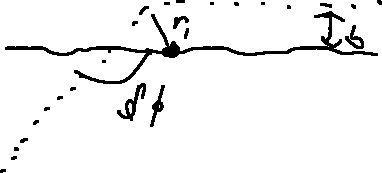
\includegraphics[width=6cm]{2-06-1.png}
	\caption*{Deflection of light}
\end{figure*}

We can then see:
\begin{align*}
	\Delta \phi &= 2\int_{r_1}^\infty \frac{dr}{r^2\sqrt{\frac{1}{b^2} - W_\text{eff}}}
\end{align*}
At our turning point $\frac{1}{b^2} = W_\text{eff}$, we can do a change of variables $r= \frac{b}{w}$:
\begin{align*}
	\Delta \phi &= 2\int_{0}^{w_1} \frac{dw}{\sqrt{1 - w^2\left(1- \frac{2M}{b}w\right)}}
\end{align*}
We can evaluate our value of $b$ which should be approximately the radius of the sun, and clearly $M$ is just the mass of the sun, so we find $\frac{2M}{b} \approx 10^{-6}$.
Therefore we should be find to expand in terms of $\frac{2M}{b}$:
\begin{align*}
	\Delta \phi &= 2\int_{0}^{w_1} \frac{dw}{\sqrt{1- \frac{2M}{b}w}\sqrt{\left(1- \frac{2M}{b}w\right)^{-1} - w^2}} \\
	\Delta \phi &= 2\int_{0}^{w_1} \frac{dw(1+ \frac{Mw}{b})}{\sqrt{1+ \frac{2M}{b}w - w^2}} \\
	\Delta \phi &= \pi + \frac{4M}{b} \\
	\delta\phi &= \delta\phi - \pi \\
	\delta\phi &= \frac{4GM}{c^2b}
\end{align*}
Which for the sun we see $\delta\phi \approx 1.7"$. This provides a measurable difference in the path that light takes.

Additionally we can see that we see a time delay for the passage of light compared to flat spacetime. 
We construct this in terms of a ranging experiment.
\begin{figure*}[h]
	\centering
	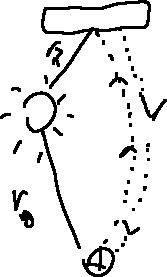
\includegraphics[width=4cm]{2-06-2.png}
	\caption*{Ranging experiment}
\end{figure*}

We see:
\begin{align*}
	e&= \left(1- \frac{2M}{r}\right)\frac{dt}{d\lambda} \\
	\frac{dt}{d\lambda} &= \left(1 - \frac{2M}{r}\right)^{-1} e \\
	\frac{dt}{dr} &= \pm \frac{1}{b}\left(1-\frac{2M}{r}\right)^{-1} \left[ \frac{1}{b^2} - W_\text{eff}\right]^{-\frac{1}{2}}
\end{align*}
And:
\begin{align*}
	\Delta t &= 2t(r_\oplus,r_1) + 2t(r_r,r_1) \\
	t(r,r_1) &=\int_{r_1}^r \frac{dr}{b}\left(1-\frac{2M}{r}\right)^{-1} \left[ \frac{1}{b^2} - W_\text{eff}\right]^{-\frac{1}{2}}
\end{align*}
We look only to first order in $M$ so we see:
\begin{align*}
	b &= r_1\left(1 - \frac{2M}{r_1}\right)^{-\frac{1}{2}} \\
	b &\approx r_1 + M
\end{align*}
So then we can see:
\begin{align*}
	t(r,r_1) &= \sqrt{r^2 - r_1^2} + 2M \log\frac{r+ \sqrt{r^2 - r_1^2}}{r_1} + M \frac{r-r_1}{r+r_1}
\end{align*}
Where the classical time is clearly $\sqrt{r^2 - r_1^2}$. So our excess time is then:
\begin{align*}
	\Delta t_\text{excess} &= \Delta t - 2\sqrt{r_\oplus^2 - r_1^2} - 2\sqrt{r_R^2  -r_1^2} \\
	\Delta t_\text{excess} &\approx \frac{4GM}{c^3} \left[\log\left(\frac{4r_Rr_\oplus}{r_1^2}\right) + 1\right]
\end{align*}
We call this the Shapiro time delay.

This time delay is important for binary star systems with pulsars and neutron stars.

\subsection{Paramaterized post-newtonian(PPN) framework}
We start with a generalized static spherically symmetric line element:
\begin{align*}
	ds^2 -A(r)dt^2 + B(r) dr^2 + r^2(d\theta^2 + \sin^2\theta d\phi^2)
\end{align*}
Where in these functions $A$ and $B$ we have a systematic way to introduce curvature from mass. In order to compare to Newtonian mechanics we do expansions in $\frac{1}{c}$ that give us Newtonian mechanics plus a correction term.
We assume that $M$ is the only parameter that influences our spacetime, so our expansion must be in terms of $\frac{GM}{c^2 r}$.
\begin{align*}
	A(r) &= 1 - \frac{2GM}{Pc^2 r} + \ldots \\
	B(r) &= 1 + \ldots
\end{align*}
We introduce parameters:
\begin{align*}
	A(r) &= 1 - \frac{2GM}{c^2 r} + 2(\beta - \gamma)\left(\frac{GM}{c^2 r}\right)^2  + \ldots \\
	B(r) &= 1 + 2\gamma \frac{GM}{c^2 r} + \ldots
\end{align*}
Where we will recover GR if $\gamma = \beta = 1$. We can think of this as $\gamma$ controlling how much space curvature ($g_{ij}$) is produced by a unit rest mass, and $\beta$ determines how much non-linearity there is in the superposition law for gravity ($g_{00}$).
We can alos introduce a $\beta_1$ that controls how much gravity is produced by unit kinetic energy and a $\beta_2$ which controls how much gravity is produced by unit gravitational potential energy, etc.
The convention is that GR is recovered when all parameters are equal to $1$.

We have constrained these experimentally to be:
\begin{align*}
	|\gamma-1| &\leq 2.3\time 10^{-5} \\
	|\beta - 1| &\leq 8\time 10^{-5}
\end{align*}
